\documentclass{article}
\usepackage{iclr2027_conference,times}

\input{math_commands.tex}

\usepackage[colorlinks=true,linkcolor=black!70!blue,citecolor=black!70!blue,urlcolor=black!70!blue]{hyperref}
\usepackage{url}
\usepackage{graphicx}
\usepackage{booktabs}
\usepackage{xcolor}
\usepackage{enumitem}
\usepackage{amsmath,amssymb,amsfonts,amsthm}
\usepackage{microtype}
\usepackage{multirow}

% Draft markers. Every marker names the evidence needed to remove it.
\definecolor{tbdcol}{HTML}{C0561B}
\newcommand{\tbd}[1]{{\color{tbdcol}\textbf{TBD}~#1}}
% Estimated number awaiting a run; the ledger in App. H gives its basis and the
% job that replaces it.
\definecolor{estcol}{HTML}{1F5FAF}
\newcommand{\est}[1]{{\color{estcol}#1$^{\dagger}$}}
\newcommand{\sieve}{\textsc{Sieve}}
\newcommand{\gplus}{G_{+}}

% Theorem-like environments used by appendix.tex.
\theoremstyle{definition}
\newtheorem{definition}{Definition}[section]
\newtheorem{theorem}{Theorem}[section]
\newtheorem{remark}{Remark}[section]

\title{When Does Joint Key-Cache Allocation Pay?\\
Output-Distortion Regimes and Their Limits on End Tasks}

\author{Anonymous authors \\ Paper under double-blind review}

% \iclrfinalcopy
\begin{document}

\maketitle

\begin{abstract}
A KV-cache budget can be spent by quantizing every token, by evicting tokens, or by mixing zero and finite precisions across tokens.  Hybrid systems already exist; we ask \emph{when} the mixed interior improves over its two endpoints, and whether the answer measured on attention-output distortion carries over to end tasks.  Under a separable local surrogate, key-token precision becomes a discrete rate-allocation problem that contains eviction as a zero-rate tier, and a finite-bit tier is dominated when its absolute logit-noise cost exceeds that of zero rate.  The fraction of heads with a dominated 2-bit tier orders the interior's exactly recomputed output-error advantage across six LLMs and 25 model--context cells (Spearman $\rho=-0.978$; $-0.94$ controlling for model), but the crossing point is architecture-specific, and longer contexts move a fixed model toward the eviction corner.  Over 4,096 decode tokens, a head's best policy family is stable while its token allocation goes stale within steps.  An end-task audit against quantization and eviction baselines then bounds these findings.  The output-error-optimal allocator is the strongest \emph{token-selective} policy we test (0.77 vs.\ 0.60 mean task score), but on both end-task models a dense low-bit quantizer beats every token-selective policy once the quantizer suits the model: TurboQuant on Llama-3.1-8B (0.99 vs.\ 0.65) and per-channel KIVI or KVQuant on Qwen3-8B, where TurboQuant itself loses (8k: 0.99 vs.\ 0.95 for the allocator and 0.90 for TurboQuant).  Output distortion predicts accuracy only weakly across methods and misprices rotated quantization noise.  The allocator's dominant failure is answer truncation, which smoothing its token scores over neighboring positions largely removes (8k: 39\% to 9\% of answers).
\end{abstract}

% ===========================================================================
\section{Introduction}
\label{sec:intro}
% ===========================================================================

At long context, the KV cache can bound batch size and decode throughput.  A cache budget admits at least three actions: assign every token one low precision~\citep{liu2024kivi,hooper2024kvquant,zandieh2025turboquant}, retain selected tokens at a higher precision~\citep{zhang2023h2o,liu2023scissorhands,li2024snapkv,xiao2024streamingllm}, or mix zero and finite rates across tokens, the \emph{interior} between those two endpoints.  The last option is no longer hypothetical: DiffKV and HqeKV combine pruning with multiple precision levels~\citep{zhang2025diffkv,wang-etal-2026-hqekv}.  What remains unclear is whether the extra interior choices are useful for a given model and deployment context, whether a simpler endpoint already suffices, and whether the proxy used to design such allocators predicts what a user observes.

This paper is a measurement study of those questions.  It does not propose a better compressor.  We build the allocator that is optimal for attention-output distortion, \sieve{}, and use it as an instrument: it tells us how large the interior's advantage can be under that objective, where the advantage disappears, and whether it survives the step to task accuracy.  The motivating reversal is within one model: from 8k to 128k, the share of Llama-3.3-70B's heads whose 2-bit tier is dominated by eviction ($D_2$, \S\ref{sec:framework}) rises from $5.5\%$ to $41.4\%$, the interior's hindsight portfolio gain ($\gplus$, \S\ref{sec:protocol}) falls from $3.17\times$ to $1.40\times$, and the share of heads where the interior beats both endpoints by $2\times$ (the \emph{band}) falls from $87.4\%$ to $21.3\%$.  A verdict at one context therefore need not transfer to another.

\paragraph{Findings.}  We organize the paper around seven observations (Table~\ref{tab:findings}).  F1--F3 concern attention-output distortion, where the interior is well defined and exactly measurable (\S\ref{sec:regimes}).  F4--F6 test whether those regimes transfer to retrieval accuracy against published quantization and eviction baselines (\S\ref{sec:endtask}); the answer is mixed, and the way it fails is informative.  F7 cuts across both levels: the comparison itself moves verdicts more than sampling does.

\begin{table}[t]
\centering
\small
\setlength{\tabcolsep}{4pt}
\caption{Summary of findings, their evidence, and what they do \emph{not} show.}
\label{tab:findings}
\begin{tabular}{@{}p{0.03\linewidth}p{0.40\linewidth}p{0.20\linewidth}p{0.29\linewidth}@{}}
\toprule
& \textbf{Observation} & \textbf{Evidence} & \textbf{Boundary} \\
\midrule
F1 & Tier extinction ($D_2$) orders the interior's output-error advantage & 25 cells, $\rho=-0.978$; Fig.~\ref{fig:regime}a & crossing is per architecture, not universal \\
F2 & Longer context moves a fixed model toward the eviction corner & 6 trajectories, 4k--256k; Fig.~\ref{fig:regime}b & mostly absolute length, small RoPE-cap residual \\
F3 & Policy family is slow; token allocation is fast & 6 cells, 4,096 tokens; Fig.~\ref{fig:evidence}b & output error only \\
F4 & The output-error optimum is the strongest token-selective policy, but a model-matched dense quantizer beats all of them & 36 task cells (7 methods) + 14 at 8k (all 13); Table~\ref{tab:endtask}, Fig.~\ref{fig:endtask}a & best quantizer differs by model; 32k/128k rerun pending \\
F5 & Output distortion ranks budgets and contexts well and methods weakly & within-cell $\rho=-0.36$ (8k, 11 methods); Fig.~\ref{fig:endtask}b & misprices rotated noise; full grid pending \\
F6 & Token-granular allocation truncates multi-token answers; positional smoothing largely repairs it & 36\% vs.\ 1--11\% (128k); 39\% $\to$ 9\% (8k); Fig.~\ref{fig:endtask}c & pre-registered 128k test pending \\
F7 & The comparison set and information contract move verdicts more than prompt sampling does & 4 contrasts; Table~\ref{tab:contract} & 4 cells for the sampling estimate \\
\bottomrule
\end{tabular}
\vspace{-2mm}
\end{table}

\paragraph{Contributions.}
\begin{enumerate}[leftmargin=*,itemsep=1pt,topsep=2pt]
  \item \textbf{A common action space and a measurable coordinate.} We place within-head key-token precision and eviction under one local output-distortion surrogate, keep the exact set-eviction error distinct from its separable zero-rate approximation, and derive a tier-extinction coordinate $D_2$ (\S\ref{sec:framework}).
  \item \textbf{A regime map for output distortion.} With exact recomputation and a symmetric information contract, we show where the interior pays, how context moves a model across regimes, and on which two timescales a controller would have to act (F1--F3).
  \item \textbf{An end-task audit of the map.} Against quantization and eviction baselines at matched key bits, we identify where output-distortion optimality transfers to task accuracy, where it does not, and the mechanism of the largest failure (F4--F6).
\end{enumerate}

Concurrent RDKV also derives joint eviction--quantization rate allocation~\citep{zhang2026rdkv}.  Our contribution is complementary: we measure \emph{when} a token-precision interior lowers attention-output error, how that changes with context, and how far that proxy carries to task accuracy.  Section~\ref{sec:related} compares with RDKV and other allocation axes.

% ===========================================================================
\section{Joint token-rate allocation as a common foundation}
\label{sec:framework}
% ===========================================================================

\paragraph{Scope and local quantization surrogate.}
For one query $q$, keys $k_i$, and values $v_i$, let
$s_i=q^\top k_i/\sqrt d$, $a=\operatorname{softmax}(s)$, and
$o=\sum_i a_i v_i$.  Quantizing key $i$ perturbs its logit by $\delta_i$, and the first-order output change is $\Delta o \approx \sum_i a_i(v_i-o)\delta_i$.
If residual perturbations are zero mean and cross-token covariance terms vanish,
\begin{equation}
  \mathbb E\|\Delta o\|^2
  \approx \sum_i w_i d_{b_i}, \qquad
  w_i=a_i^2\|v_i-o\|^2,\quad d_b=\operatorname{Var}(\delta_b).
  \label{eq:surrogate}
\end{equation}
Only a common-mode logit shift is canceled exactly by softmax; token-dependent bias and covariance are outside this surrogate.  We therefore use Eq.~\ref{eq:surrogate} to \emph{choose} allocations, never to score their reported error.

\paragraph{Exact eviction versus a zero-rate surrogate.}
For an evicted set $E$ with mass $A_E=\sum_{i\in E}a_i$, renormalizing the surviving attention gives exactly
\begin{equation}
 \|o_{\setminus E}-o\|^2
 =\frac{\left\|\sum_{i\in E}a_i(v_i-o)\right\|^2}{(1-A_E)^2}.
 \label{eq:exact-eviction}
\end{equation}
The denominator and cross-token inner products make set eviction nonseparable; for a singleton $j$ the magnitude is $a_j\|v_j-o\|/(1-a_j)$, as derived by CAOTE~\citep{goel2025caote}.
To include zero rate in a token-separable allocator, we use the small-evicted-mass, cross-term-free approximation
$\widetilde D_0(E)=\sum_{i\in E}w_i$ and normalize its \emph{absolute} cost to $d_0=1$.  Eviction is therefore a zero-rate action \emph{inside the surrogate}, not an exact independent-token equality.

\paragraph{The implemented discrete allocation.}
For tiers $\mathcal B=\{0,1,2,3,4,5,6,8\}$ and an average key budget $B$, we solve
\begin{equation}
 \min_{b_i\in\mathcal B}\sum_i w_i d_{b_i}
 \quad\text{s.t.}\quad \sum_i b_i\le BL,
 \qquad
 b_i^\star(\lambda)=\arg\min_{b\in\mathcal B}\{w_i d_b+\lambda b\},
 \label{eq:discrete}
\end{equation}
with a bisection on $\lambda$ enforcing the budget.  Relaxing bits to be continuous with $d_b\propto4^{-b}$ gives $b_i^\star=\log_2a_i+\log_2\|v_i-o\|+c$, which explains the reverse-water-filling shape; Eq.~\ref{eq:discrete} is the optimizer used in all experiments.

\paragraph{Two coordinates, not one universal phase boundary.}
If $d_b\ge d_0$, tier $b$ consumes bits without lowering the surrogate cost and is dominated.  This condition is sufficient for extinction but not necessary.  We summarize the sharp side by
\begin{equation}
 D_2=H^{-1}\textstyle\sum_{h=1}^{H}\mathbb I[d_{h,2}\ge d_0],
 \label{eq:d2}
\end{equation}
the fraction of heads in a model--context cell whose 2-bit tier is dominated.  The diffuse side is different: unequal allocation has little leverage when token importance varies less than the tier spacing.  For attention-only importance, $\operatorname{std}_i(\log_2a_i)=\tau/\ln2$ is an algebraic identity, not evidence of optimality.  Thus $D_2$ measures approach to the eviction-like corner, and a dispersion coordinate is needed for the uniform corner.  $D_2$ contains no explicit $L$, but it is measured \emph{at} a context and changes with it.

% ===========================================================================
\section{Measurement protocol}
\label{sec:protocol}
% ===========================================================================

We measure at two levels.  Attention-output distortion is exact and cheap, so it supports a dense regime map over six models and 4k--256k tokens (\S\ref{sec:regimes}).  End-task accuracy is the quantity users observe but is expensive, so we audit the map on two models chosen to lie at opposite ends of it, with a third pending (\S\ref{sec:endtask}).

\paragraph{Output-distortion level: models, cells, and units.}
We evaluate Llama-3.1-8B and Llama-3.3-70B~\citep{grattafiori2024llama3}, Mistral-7B~\citep{jiang2023mistral}, Qwen1.5-MoE-A2.7B~\citep{qwen2024moe}, Qwen3-8B, and Qwen3-30B-A3B~\citep{yang2025qwen3}.  A symmetric grid has 16 model--context cells between 8k and 128k, and its extension has 25 cells spanning 4k--256k (44,416 query-head--configuration aggregates).  Across the six architectures there are 10,240 query-head and 2,016 KV-head positions, reused across contexts, so statistical claims treat cells and models, not heads, as independent units.  PG-19 text~\citep{rae2020pg19} supplies the haystack, and every cell passes a full-cache needle-retrieval gate.

\paragraph{Compression, budget, and information contract.}
Keys are quantized with TurboQuant$_{\rm mse}$~\citep{zandieh2025turboquant} (random rotation and Lloyd--Max scalar quantization~\citep{lloyd1982least}).  The headline budget is $B=3$ key bits per context token; tier 0 evicts and tier 8 stores an 8-bit key.  Values remain uncompressed.  The primary comparison is symmetric: the mixed allocator and the eviction endpoint both use only lagged attention, and positions unseen by that score stay at the maximum tier.  The endpoints, which we also call \emph{corners}, are uniform 3-bit quantization and accumulated-attention eviction keeping the number of 8-bit keys the budget allows (\emph{uniform+accum}); a robustness analysis takes the minimum over five corners.  Oracle results are upper bounds only.

\paragraph{Exact response and metrics.}
For every assignment we quantize the real keys, recompute attention, and measure the output error exactly.  For head $h$,
\begin{equation}
 g_h=\frac{\min(D_h^{\rm uniform},D_h^{\rm evict})}{D_h^{\rm mixed}},
 \qquad
 \gplus=\exp\!\left[H^{-1}\textstyle\sum_h\log\max(g_h,1)\right].
 \label{eq:metrics}
\end{equation}
$\gplus$, the primary cell response, is a hindsight portfolio statistic, not achieved router performance.  The share of heads with $g_h\ge2$ (the band) is a secondary summary, with predeclared thresholds: a cell is GO when its band is at least 35\%, STOP below 15\%, and NARROW in between.

\paragraph{End-task level.}
Llama-3.1-8B (8k, 32k, 128k) and Qwen3-8B (8k, 32k) share size and GQA ratio but sit at opposite ends of the map (low vs.\ high $D_2$).  Four RULER-style tasks~\citep{hsieh2024ruler} (single-needle, multi-key, multi-value retrieval, and variable tracking) use 20 held-out prompts per cell.  The cache is compressed once, after the context is prefilled and \emph{before} the question arrives, as in prefix caching; compressing after the question lets observation-window scores read it and saturates every such method at 1.00.  Budgets are $B\in\{2,3\}$ key \emph{code} bits per context token, audited at run time; values, the last 32 context tokens, and generated tokens are uncompressed in every method.  Side information (norms, scales, outlier indices, width maps) is reported as effective bits.  Blocks where the uncompressed model scores below 0.9 are excluded (only Qwen3-8B multi-value), leaving 36 valid model/context/task/budget cells.  Mistral-7B (8k, 32k), which shares the GQA ratio and sits on Llama's side of the map, is being added as a third model under the same protocol.

\paragraph{Baselines and the instrument.}
Quantization: TurboQuant-MSE, KIVI~\citep{liu2024kivi}, and KVQuant~\citep{hooper2024kvquant}.  Eviction, all keeping $\lfloor BC/8\rfloor$ 8-bit keys: H2O~\citep{zhang2023h2o}, SnapKV~\citep{li2024snapkv}, DropKV~\citep{zhang2026dropkv}, Ada-KV~\citep{feng2024adakv}, LaProx~\citep{mai2026laprox}, and OBCache-K~\citep{gu2026obcache} with Ada-KV allocation.  \sieve{} is Eq.~\ref{eq:discrete} per KV head with a 4-bit cascade score (\S\ref{sec:regimes}), plus a router that assigns each KV head to the mixed interior, uniform quantization, or eviction by minimum output error on 10 disjoint calibration prompts.  \sieve{}'s router is therefore \emph{output-error-optimal by construction}; its end-task behavior tests the proxy, not a tuned method.  Implementation details and deviations are in Appendix~\ref{app:endtask}.

% ===========================================================================
\section{Output-distortion regimes}
\label{sec:regimes}
% ===========================================================================

\begin{figure}[t]
  \centering
  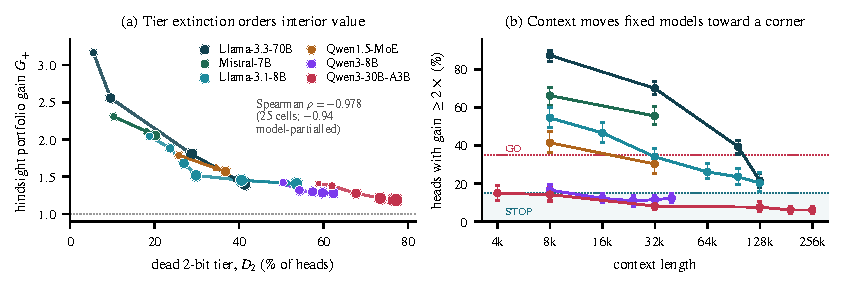
\includegraphics[width=\linewidth]{figures/fig1_regime.pdf}
  \vspace{-4mm}
  \caption{\textbf{F1--F2: where the interior lowers output error.} Mixed allocator and eviction endpoint both use lagged information; exact recomputation scores both. \textbf{(a)} The tier-extinction coordinate $D_2$ orders hindsight portfolio gain $\gplus$ across 25 cells; arrows show increasing context. \textbf{(b)} Context moves each fixed model across predeclared output-error bands. Error bars are 90\% layer-cluster intervals. Thresholds are not universal across architectures.}
  \label{fig:regime}
  \vspace{-3mm}
\end{figure}

\paragraph{F1: Tier extinction orders the interior's value, but the crossing is per architecture.}
On the 16-cell grid, demoting both the mixed allocator and the eviction endpoint to lagged information retains roughly half of the apparent asymmetric advantage (Fig.~\ref{fig:evidence}a): the symmetric band stays $1.2$--$12.5$ points above the all-oracle band in all 16 cells, five cells fall below 15\% (STOP), and $\gplus$ ranges from $1.05\times$ to $3.21\times$.  $D_2$ still orders the symmetric band at $\rho=-0.985$.  Extending to 25 cells, $D_2$ has Spearman $\rho=-0.978$ with both $\gplus$ and the band, and $-0.94$ with $\gplus$ ($-0.915$ with the band) after partialling out model identity (Fig.~\ref{fig:regime}a).  The crossing, however, is not universal.  Pooled monotone crossings sit near $D_2=29.0\%$ (GO) and $54.1\%$ (STOP), yet Llama-3.1-8B holds $20.2\%$ band at $D_2=53.7\%$ while Qwen3-8B is at $12.2\%$ at $D_2=54.3\%$, an eight-point gap across $0.6$ points of $D_2$ that exceeds prompt uncertainty.  $D_2$ is an ordering coordinate; any operational boundary must be fitted per architecture.  The location also depends on what information each side of the comparison receives: on the same 16 cells, STOP is crossed at $D_2=46.9\%$ when both sides see the current query and at $57.4\%$ when both use lagged attention, a $10.5$-point shift larger than either confidence interval, and under the asymmetric contract it is never crossed.  $D_2$ itself does not share this sensitivity: across two campaigns with different corner sets and code it agrees to within $0.30$ points on all 15 shared cells.  How much the band depends on the comparison is taken up in F7.

\paragraph{Why $D_2$ rather than a concentration or context statistic?}
We compared $D_2$ with simpler predictors on the same 25 cells, under a protocol fixed before computing it (Table~\ref{tab:app-predictors}): attention concentration $\tau$, the spread of log token sensitivity (a heterogeneity statistic of the kind RateQuant uses~\citep{zuo2026ratequant}), attention entropy, and context length alone.  Within a model, every statistic that moves with context orders $\gplus$ almost perfectly (mean within-model $\rho=-0.99$ for $D_2$, $\tau$, the heterogeneity statistic, and context length).  The difference is across architectures.  Pooled over models, $D_2$ reaches $\rho=-0.978$, against $-0.72$ for $\tau$ and heterogeneity and $-0.48$ for context alone, and a log-linear fit on five models predicts the sixth to within a factor of $1.12$ for $D_2$, against $1.15$ and $1.24$.  $D_2$ is therefore most useful for comparing architectures, and its held-out advantage over dispersion statistics is modest.

\paragraph{F2: Context moves a fixed model toward the eviction corner.}
Every measured trajectory moves toward larger tier extinction with context (Fig.~\ref{fig:regime}b).  Llama-3.3-70B goes from GO at 8k to NARROW at 128k; Qwen3-8B goes from NARROW at 8k to STOP by 16k.  The mechanism is mostly absolute length: attention concentration $\tau$ is generally convex in $\log L$.  Reaching the trained RoPE cap adds a residual of about $+0.21$ in Qwen3-8B and Qwen3-30B, but none in Llama-3.1-8B and none at $0.75$ of the cap.  Both context and architecture matter; the data do not support a universal RoPE-triggered transition.  The surrogate that drives these allocations is useful but not exact: the median ratio of predicted to exactly recomputed gain lies in $[0.79,1.34]$ across the configuration grid, which we treat as model-fit validation rather than held-out prediction.

\begin{figure}[t]
  \centering
  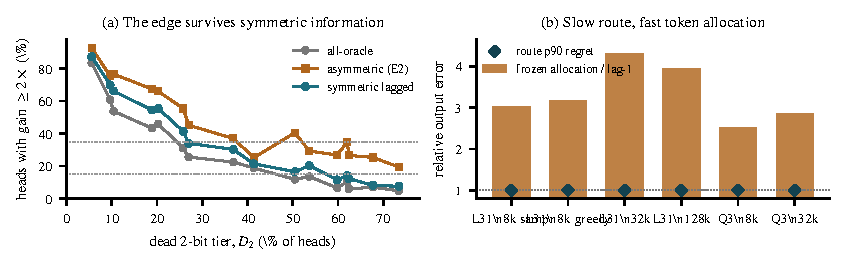
\includegraphics[width=\linewidth]{figures/fig2_evidence.pdf}
  \vspace{-4mm}
  \caption{\textbf{F1 robustness and F3 timescales.} \textbf{(a)} On the same 16 cells, the lagged-versus-lagged advantage is smaller than the asymmetric estimate (current-query interior against lagged eviction) but remains ordered by $D_2$. \textbf{(b)} In six cells, keeping the calibration-time \emph{policy family} has p90 regret $1.00$ through 4,096 generated tokens, whereas freezing the token assignment costs $2.52$--$4.30\times$ a one-step-old assignment.}
  \label{fig:evidence}
  \vspace{-3mm}
\end{figure}

\paragraph{F3: Two timescales, and the cost of acting on them.}
A head's output-error-optimal family (interior, uniform, or eviction) is stable over 4,096 generated tokens in all six measured cells, while the token allocation inside a mixed head goes stale within steps (Fig.~\ref{fig:evidence}b).  Any controller built on this map must therefore route rarely but re-budget often.  Table~\ref{tab:deployment} prices the two constraints such a controller meets.  These are output-error results; \S\ref{sec:endtask} tests whether they matter for accuracy.

\begin{table}[t]
\centering
\small
\setlength{\tabcolsep}{4pt}
\caption{Measured costs of acting on the output-distortion map. Output error only.}
\label{tab:deployment}
\begin{tabular}{@{}p{0.29\linewidth}p{0.25\linewidth}p{0.38\linewidth}@{}}
\toprule
\textbf{Constraint} & \textbf{Measurement} & \textbf{Implication} \\
\midrule
Family label over 4,096 tokens & p90 regret $1.00$ in 6/6 cells & calibrate the route once per context \\
Frozen token assignment & $2.52$--$4.30\times$ lag-1 error & re-budget mixed heads every few steps \\
Shared GQA allocation & $1.000/1.136/1.316\times$ at $n_{\rm rep}=1/4/8$ & route per KV head at a small cost \\
4-bit current-query cascade & closes $82$--$91\%$ (median $89\%$) of lag penalty & re-score from base-tier keys \\
\bottomrule
\end{tabular}
\vspace{-2mm}
\end{table}

% ===========================================================================
\section{Do output-distortion regimes transfer to end tasks?}
\label{sec:endtask}
% ===========================================================================

\begin{table}[t]
\centering
\footnotesize
\setlength{\tabcolsep}{2.6pt}
\caption{\textbf{End-task audit} (mean RULER score over valid cells; FP $=0.999$). \emph{Full grid}: the 36 valid cells (Llama-3.1-8B 8k/32k/128k, Qwen3-8B 8k/32k, four tasks, $B\in\{2,3\}$), one run per cell. \emph{8k rerun}: all methods in one process per cell on the same prompts, 14 valid cells (measured). Output error and effective bits ($B=2$, code bits plus side information) are from the 8k rerun. \emph{Hard}: Llama-3.1-8B, 32k, 32-key retrieval, $B=2$. \est{Blue} numbers are estimates awaiting runs (App.~\ref{app:ledger}).}
\label{tab:endtask}
\begin{tabular}{@{}llrrrrrrrr@{}}
\toprule
& & \multicolumn{3}{c}{full grid (36 cells)} & \multicolumn{2}{c}{8k rerun (14 cells)} & & & \\
\cmidrule(lr){3-5}\cmidrule(lr){6-7}
family & method & Llama & Qwen & all & Llama & Qwen & out.\ err. & eff.\ bits & hard \\
\midrule
\multirow{4}{*}{quant.} & TurboQuant-MSE & \textbf{0.985} & 0.867 & 0.946 & \textbf{0.997} & 0.895 & 0.439 & 2.12 & \est{0.88} \\
 & KIVI ($g{=}128$) & \est{0.96} & \est{0.97} & \est{0.96} & 0.964 & 0.987 & 0.300 & 2.25 & \est{0.85} \\
 & KIVI ($g{=}32$) & \est{0.98} & \est{0.99} & \est{0.98} & 0.986 & \textbf{1.000} & 0.203 & 3.00 & \est{0.88} \\
 & KVQuant & \est{0.97} & \est{0.98} & \est{0.97} & 0.976 & 0.990 & \textbf{0.163} & 2.33 & \est{0.88} \\
\midrule
\multirow{6}{*}{eviction} & H2O & \est{0.38} & \est{0.33} & \est{0.36} & 0.354 & 0.358 & 0.341 & 2.04 & \est{0.25} \\
 & SnapKV & 0.479 & 0.237 & 0.398 & 0.348 & 0.203 & 0.324 & 2.04 & \est{0.21} \\
 & DropKV & 0.459 & 0.334 & 0.418 & 0.331 & 0.262 & 0.345 & 2.04 & \est{0.18} \\
 & Ada-KV & 0.612 & 0.285 & 0.503 & 0.464 & 0.233 & 0.326 & 2.04 & \est{0.25} \\
 & LaProx & 0.640 & 0.457 & 0.579 & 0.540 & 0.455 & 0.330 & 2.04 & \est{0.32} \\
 & OBCache-K + Ada-KV & 0.719 & 0.369 & 0.602 & 0.580 & 0.298 & 0.334 & 2.04 & \est{0.39} \\
\midrule
\multirow{2}{*}{mixed} & \sieve{} interior only & 0.479 & 0.438 & 0.465 & 0.467 & 0.508 & 0.165 & 2.07 & \est{0.28} \\
 & \sieve{} (router) & 0.654 & \textbf{0.989} & 0.766 & 0.680 & 0.953 & 0.150 & 2.08 & \est{0.32} \\
\midrule
\multirow{2}{*}{diag.} & \sieve{}, pooled score & --- & --- & --- & 0.779 & 0.633 & 0.196 & 2.07 & --- \\
 & \sieve{}, oracle router & --- & --- & --- & 0.834 & 0.967 & 0.136 & 2.08 & --- \\
\bottomrule
\end{tabular}
\vspace{-2mm}
\end{table}

\tbd{[R12-A] Paired rerun: 8k measured (Table~\ref{tab:endtask}); Llama 32k and 128k and Qwen 32k pending. Once complete it replaces the full-grid columns and Fig.~\ref{fig:endtask}, because the forward pass is not bit-reproducible across runs. [R12-B] Hard cell, 60 fresh prompts; pre-registered gate: FP $\ge0.95$ and TurboQuant in $[0.50,0.90]$. On its 10 calibration prompts FP and TurboQuant both score 0.90, so the gate may fail. [R12-C] Question-visible control: measured except Llama 128k. [R12-D] Mistral-7B evaluation pending.}

\paragraph{F4: The output-error optimum is the strongest token-selective policy, but a model-matched dense quantizer beats all of them.}
Table~\ref{tab:endtask} and Fig.~\ref{fig:endtask}a show three regularities.  First, among policies that choose \emph{which tokens} to keep, \sieve{} scores highest: 0.766 against 0.602 for OBCache-K + Ada-KV over the full grid ($+0.16$, 90\% CI $[+0.13,+0.20]$ by prompt bootstrap), and in the 8k rerun it beats every eviction method, including H2O, on average (0.797 against at most 0.504) with less than half their output error.  Second, on Llama-3.1-8B, keeping every token at low precision dominates: TurboQuant scores 0.985, and at $B=2$ every token-selective method trails it by at least $0.35$ (best: OBCache-K + Ada-KV, 0.626 vs.\ 0.976; \sieve{}, 0.429).  Third, on Qwen3-8B, TurboQuant's per-token rotated 2-bit keys break down (variable tracking scores $0.46$ at 8k and $0.40$ at 32k) and \sieve{} beats it (0.989 vs.\ 0.867).  That reversal belongs to the quantizer, not to dense quantization.  In the 8k rerun the per-channel quantizers recover Qwen: KIVI scores 0.987 at $g{=}128$ and 1.000 at $g{=}32$, and KVQuant 0.990, all above \sieve{} (0.953), with KIVI-128 and KVQuant using only 0.17--0.25 more effective bits.  On Llama the order of the quantizers reverses (TurboQuant 0.997, KIVI-128 0.964).  So on both models some dense quantizer beats every token-selective policy, but which one depends on the model.  Mistral-7B looks like Llama on its calibration prompts (TurboQuant 0.93--1.00, SnapKV 0.03--0.10, \sieve{}'s interior 0.00--0.27); its evaluation is pending (\sieve{} router \est{0.55}).  The regime map predicts that the gain from the interior differs across architectures (F1); it does not predict whether a dense quantizer does better still.  The preregistered correlation between the output-error band and the router's accuracy gain is $-0.70$, opposite in sign to the prediction.  All 15 full-grid cells where \sieve{} loses to an eviction method are on Llama: 7 of 8 at $B=2$ below 128k, and all 8 at 128k (Table~\ref{tab:app-h2h}).

\begin{figure}[t]
  \centering
  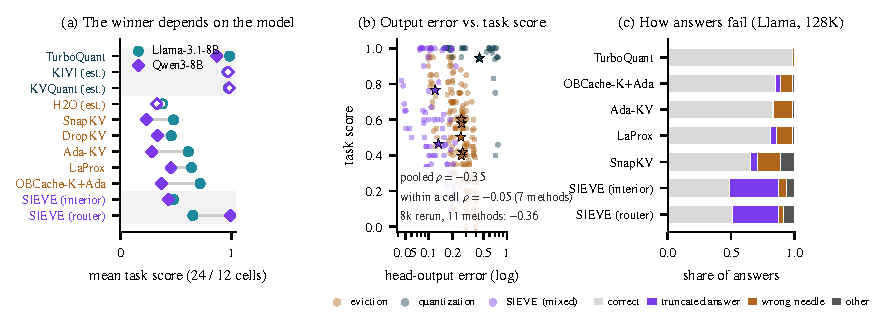
\includegraphics[width=\linewidth]{figures/fig3_endtask.pdf}
  \vspace{-4mm}
  \caption{\textbf{F4--F6: what transfers to task accuracy.} \textbf{(a)} Mean task score per method and model; hollow markers are estimates awaiting runs (App.~\ref{app:ledger}). Full-grid means; KIVI, KVQuant and H2O are full-grid estimates guided by the 8k rerun (Table~\ref{tab:endtask}). TurboQuant wins on Llama-3.1-8B; on Qwen3-8B \sieve{} beats TurboQuant but not the per-channel quantizers. \textbf{(b)} Head-output error vs.\ task score for every full-grid (cell, method); stars are method means. Error tracks accuracy across budgets and contexts; across methods it is weak, and TurboQuant (dark, top right) combines the highest error with the highest accuracy. \textbf{(c)} Single- and multi-key answers at Llama-3.1-8B, 128k, $B\in\{2,3\}$: \sieve{} fails by \emph{truncating} the correct number, eviction methods by returning a wrong needle.}
  \label{fig:endtask}
  \vspace{-3mm}
\end{figure}

\paragraph{F5: Output distortion ranks budgets and contexts well and methods weakly.}
\sieve{} minimizes the distortion it targets and has among the lowest head-output errors (0.120 on the full grid, 0.150 in the 8k rerun), yet dense quantizers beat it.  Fig.~\ref{fig:endtask}b separates the two uses of the proxy.  Across budgets and contexts, error and accuracy move together ($\rho=-0.69$ within the eviction family on the full grid).  Across methods at a fixed budget the relation is weak and depends on which methods are compared.  With the seven full-grid methods, the mean within-cell rank correlation is $-0.05$; with all eleven methods of the 8k rerun it is $-0.36$ ($-0.46$ among token-selective policies, and $0.01$ among the four dense quantizers).  The exception that breaks the proxy is TurboQuant: its rotated, spread-out noise gives the highest output error (0.44) at the highest Llama accuracy, while per-channel quantizers have low error and high accuracy.  Output distortion therefore sizes budgets but misprices at least one quantizer family, and it should not choose between families.  \tbd{[R12-A] Recompute these correlations on the full paired grid.}  The router's calibration costs part of its accuracy but is not the main culprit: routing each head on its \emph{measured} test-prompt error raises the 8k score from 0.797 to 0.891 (Llama: 0.680 to 0.834), still below every dense quantizer; at Llama-3.1-8B 32k, $B=2$ the same oracle trails TurboQuant by 0.20 (90\% CI $[-0.32,-0.09]$) while sending 93\% of heads to the interior.  The allocation theorem holds for its own objective; the transfer from that objective to retrieval is what fails.

\paragraph{F6: Token-granular allocation truncates multi-token answers.}
\sieve{}'s weakest setting is Llama-3.1-8B at 128k, where it trails OBCache-K + Ada-KV by $0.32$ at $B=2$ (0.442 vs.\ 0.762).  Its wrong answers have a distinctive form (Fig.~\ref{fig:endtask}c).  Asked for 4929054 it answers ``492''; for 9465170, ``946''; for 6022964, ``602296''.  Llama tokenizes digits in groups of three, so the allocator keeps the key and the first token of the value and loses the tokens after it.  Truncation accounts for 36\% of \sieve{}'s single- and multi-key answers at 128k (39\% for the interior alone) against 1--11\% for every eviction method, which instead fail by returning a different needle (10--18\%).  Truncation is not specific to 128k: pooled over Llama's three contexts, 40\% of the interior's answers are truncated.  The router does not rescue these heads, because by its objective the interior is the right choice: at 128k it sends 99\% of Llama's KV heads to the interior, whose output error (0.094) is half that of any eviction method.  Losing the second token of one needle's value barely moves an error averaged over heads and answer steps, but changes the answer completely.

Why do the eviction methods avoid truncation?  Every one of them that beats \sieve{} here smooths its token score over neighboring positions before selecting (max- or average-pooling over 7 positions), so a kept token protects its neighbors and a needle survives as a phrase.  Pooling has its own cost: with several targets it can merge evidence that belongs to different ones~\citep{zhang2026fixedcontract}.  \sieve{} allocates each token independently from unpooled attention.  We pre-registered a test of this explanation: the same water-filling allocator on pooled attention supports it if it recovers at least half of the 128k, $B=2$ gap to OBCache-K + Ada-KV, and refutes it below one fifth.  The 8k rerun already points strongly in that direction.  On Llama-3.1-8B single- and multi-key retrieval, pooling cuts truncated answers from 39\% to 9\% and raises the interior's score from 0.467 to 0.779, above OBCache-K + Ada-KV (0.580) and the calibrated router (0.680); at $B=2$ it moves the interior from 0.299 to 0.663, past OBCache's 0.446.  On Qwen3-8B pooling helps less (0.508 to 0.633; router 0.953).  The pre-registered 128k cell remains the test (estimate \est{0.58}; half-gap threshold 0.59; oracle router \est{0.55}).  \tbd{[R12-A, diagnostic arms] interior\_pool and router\_oracle at 128k.}

\paragraph{F7: Verdicts depend more on the comparison than on the sample.}
Across both levels, the largest changes in a verdict came from what a method was compared against, and under which information contract, rather than from which prompts were drawn (Table~\ref{tab:contract}).  A new prompt block moves the band by a standard deviation of only $0.4$--$3.0$ points, so six prompts per cell suffice.  Each of the four other choices in Table~\ref{tab:contract} moves a result by more than that and changes at least one verdict: the eviction corner, the information each side sees (F1), whether the question is visible when the cache is compressed, and which dense quantizer stands for the endpoint (F4).  A KV-compression verdict is therefore not a measurement until it names its comparison set and information contract.

\begin{table}[t]
\centering
\small
\setlength{\tabcolsep}{4pt}
\caption{\textbf{F7:} how much each choice moves a verdict, compared with prompt sampling.}
\label{tab:contract}
\begin{tabular}{@{}p{0.34\linewidth}p{0.36\linewidth}p{0.22\linewidth}@{}}
\toprule
\textbf{Choice varied} & \textbf{Effect} & \textbf{Verdicts changed} \\
\midrule
Prompt block (sampling) & band s.d.\ $0.4$--$3.0$ pts, 4 cells & none \\
Eviction corner: accum vs.\ best of 5 & band $-5.1$ to $-8.6$ pts & 3 of 4 borderline cells \\
Information: current query vs.\ lagged & STOP crossing $46.9\%\to57.4\%$ $D_2$ & boundary location \\
Question visible at compression & SnapKV $0.11$--$0.45\to1.00$ in 4 cells (same prompts); H2O $\le0.07$ & every eviction ranking \\
Dense baseline: TurboQuant vs.\ per-channel & Qwen3-8B 8k: $0.90\to0.99$--$1.00$ & \sieve{} vs.\ dense on Qwen \\
\bottomrule
\end{tabular}
\vspace{-2mm}
\end{table}


% ===========================================================================
\section{Implications}
\label{sec:implications}
% ===========================================================================

The two levels of measurement lead to five practical conclusions, each bounded by the retrieval tasks and the two end-task models measured so far.
\begin{enumerate}[leftmargin=*,itemsep=1pt,topsep=2pt]
  \item \textbf{Report dense low-bit quantization, with more than one quantizer, next to any token-selective method.}  On both end-task models a dense quantizer beats every eviction and mixed policy we test at 2--3 key bits, but a different one on each: TurboQuant on Llama-3.1-8B, per-channel KIVI and KVQuant on Qwen3-8B, where TurboQuant loses to \sieve{}.  A comparison among token-selective methods alone, or against a single quantizer, would have hidden both facts.
  \item \textbf{Use output distortion to size budgets, not to choose methods.}  It orders settings well (F1, F5) and methods weakly, and misprices rotated quantization noise (F5).  Routing between method families needs a task-aware signal.
  \item \textbf{Allocate spans, not tokens.}  Token-separable objectives cannot see that a multi-token answer is only useful whole (F6).  Smoothing the allocator's scores over neighboring positions, which leaves Eq.~\ref{eq:discrete} intact, already cuts truncation from 39\% to 9\% at 8k.
  \item \textbf{Name the comparison set and information contract with every verdict.}  They move results more than the prompt sample does (F7).
  \item \textbf{Calibrate per architecture and per context, and re-budget often.}  The regime crossing is architecture-specific and moves with context (F1, F2); token allocations go stale within steps (F3).
\end{enumerate}

\paragraph{Scope of the budget comparison.}  All methods are compared at matched key code bits, with side information reported as effective bits (Table~\ref{tab:endtask}; storage details in App.~\ref{app:endtask}).  Quantization is simulated, so we make no memory-traffic or latency claims; those depend on packed kernels, which are outside the scope of this study.

% ===========================================================================
\section{Related and concurrent work}
\label{sec:related}
% ===========================================================================

\paragraph{Dense KV quantization.}
Dense quantizers store every token at low precision: per-channel or per-token integer schemes~\citep{liu2024kivi,hooper2024kvquant}, low-rank and sparse residual correction~\citep{kang2024gear}, rotations and sketches~\citep{zandieh2024qjl,zandieh2025turboquant}, and importance-aware mixed precision~\citep{yang2024mikv,he2024zipcache}.  RateQuant allocates finite precision across K/V heads from fitted distortion curves~\citep{zuo2026ratequant}.  Block-scaled 4-bit formats now make such caches native to hardware: the MX formats~\citep{ocp2023mx} and NVFP4, whose 16-element blocks carry FP8 scales~\citep{alvarez2025nvfp4}, including an NVFP4 KV cache~\citep{alvarez2025nvfp4kv}.  Our results bear on how this endpoint is used as a baseline.  Its strength depends on the quantizer (F4): per-token rotated keys fail on Qwen3 at 2 bits where per-channel schemes are expected to hold, so a study of the interior has to report more than one dense quantizer (F7).

\paragraph{Eviction and sparse attention.}
Evictors keep recent and sink tokens~\citep{xiao2024streamingllm}, accumulate attention~\citep{zhang2023h2o,liu2023scissorhands}, use the last query~\citep{oren2024tova} or a prefill observation window~\citep{li2024snapkv}, and split budgets across layers and heads~\citep{cai2024pyramidkv,feng2024adakv}.  Output-aware scores estimate the attention-output perturbation of removing a token: exactly for a singleton~\citep{goel2025caote}, under perturbation constraints~\citep{feng2026criticalkv}, by decoupled residual-output perturbation~\citep{zhang2026dropkv}, by Optimal-Brain-Damage saliency~\citep{gu2026obcache}, through the value and output projection with a model-wide budget~\citep{mai2026laprox}, or by layer-wise reconstruction with spatial-temporal smoothing~\citep{an2026restkv}.  Query-aware sparsity keeps the whole cache and selects pages per query~\citep{tang2024quest}, and reasoning-oriented methods target long generated traces~\citep{cai2025rkv,mao2026triattention}.  We evaluate six of these families at matched key bits.  Our truncation finding (F6) suggests one reason the strongest ones work: most smooth their scores over neighboring positions, which protects multi-token spans in a way a token-separable output-error objective does not.  We do not claim first output-aware eviction; we state the separable approximation needed to put zero rate inside a finite-rate allocator.

\paragraph{Hybrid storage and rate allocation.}
The split between quantization and eviction is not strict.  DiffKV routes tokens among high precision, low precision, and pruning with an on-GPU manager~\citep{zhang2025diffkv}, and HqeKV optimizes among full precision, several quantized levels, and eviction using joint K--V importance~\citep{wang-etal-2026-hqekv}.  Concurrent RDKV assigns zero-to-finite rates to value tokens and key channels with packed decode~\citep{zhang2026rdkv}, and concurrent attention-aware transform coding applies output-aware reverse water-filling to transformed K/V channels~\citep{laus2026aatc}.  Our allocation unit is the within-head key token, and our question is not whether water-filling can be derived but when its interior pays and whether the answer survives the step to task accuracy.  Head, channel, and token axes are potentially composable (Table~\ref{tab:related}, App.~\ref{app:related}).

\paragraph{Diagnostics, evaluation contracts, and systems.}
Long-context compression is usually evaluated on synthetic retrieval~\citep{hsieh2024ruler} and on natural long-context tasks~\citep{bai2025longbenchv2}.  Closest in spirit to our study, \citet{zhang2026fixedcontract} hold an eviction selector's contract fixed (attention tensor, observation window, budget, projection rule) and vary one stage at a time, attributing failures to a mismatch between prefill and decode queries, to output-unaware scoring, or to a projection that fragments evidence across the budget, on the same three model families we use.  Their study covers eviction alone at 5--10\% retention and finds that output-aware scoring helps in most cells where it has room to.  Ours adds dense and mixed-precision policies and finds that output error fails at a different point: choosing \emph{between} families at a fixed budget (F5).  Our truncation failure (F6) is an instance of their projection stage, produced by a mixed-precision allocator rather than a selector, and F7 carries their fixed-contract principle one level up, to the baselines and information contract a verdict is stated under.  Deployed eviction also meets infrastructure constraints that our simulated study does not address: fused attention kernels never materialize the attention scores that score-based evictors read~\citep{dao2023flashattention2,shah2024flashattention3,zhang2024sageattention}, and paged allocators reclaim only empty blocks~\citep{kwon2023vllm}, so scattered survivors free little memory unless the cache is compacted~\citep{mao2026triattention}.

% ===========================================================================
\section{Limitations and conclusion}
\label{sec:conclusion}
% ===========================================================================

The evidence is deliberately scoped.  End-task results cover two 8B models (a third, Mistral-7B, is pending) and four synthetic retrieval tasks, so F4--F6 may not hold for reasoning, summarization, or long generation, where a truncated span may matter less or more.  Compression is key-only with exact values, budgets match key code bits rather than total KV bytes, and all quantization is simulated, so no memory or throughput claim is made.  The regime crossing is architecture-conditioned, and the diffuse (uniform) side of the map has less support than tier extinction.  The within-generation change of $\tau$ is underpowered at 3--6 prompts per cell and is not used.  Several end-task entries are estimates pending the runs listed in Appendix~\ref{app:ledger}.

Within that scope the picture is consistent.  Joint allocation is not uniformly useful: a tier-extinction coordinate orders when its interior lowers attention-output error, context moves a fixed model toward a corner, and a controller would face a slow family timescale and a fast allocation timescale.  On end tasks, the output-error optimum is the best way we found to choose \emph{which tokens} to keep, yet keeping \emph{all} tokens at low precision does better still once the quantizer suits the model, and output distortion cannot make that choice.  Its most visible failure, truncated answers, points to the unit of allocation, not the allocation theorem, as the next thing to change, and positional smoothing is a first working repair.

\label{main:end}

% Statements below follow the ICLR 2027 template; none counts toward the page limit.
\subsection*{AI use statement}

In this work, we used generative AI tools (an AI coding and writing assistant) for the following tasks that the ICLR policy requires us to disclose.
\emph{Method implementation:} implementing and testing the KIVI and KVQuant-style baseline quantizers, the end-task result readers, the predictor comparison, and the figure and table scripts.
\emph{Experiment-design feedback:} proposing parts of the end-task campaign, namely the harder 32-key operating point, the question-visible control, the third end-task model, the pooled-score and oracle diagnostic arms, the predictor-comparison protocol, and several of their pre-registered decision rules, all of which the authors reviewed before any run.
\emph{Hypothesis proposal and results interpretation:} proposing the positional-pooling explanation of answer truncation (F6), the cross-cutting observation on comparison contracts (F7), and interpretations of the end-task results.
\emph{Qualitative data analysis:} classifying the models' wrong answers as truncated, wrong-needle, or other by rule, from generated text.
We also used AI assistance, as the policy recommends disclosing, for editing code and job scripts, drafting and restructuring the paper (including its title and section structure), literature search and summarization, bibliography entries, and figure creation.  The estimated values marked in the paper and their stated bases were proposed with AI assistance.
We have not used generative AI tools to generate, alter, or impute measured data: every reported measurement is computed by the experiment code from model runs.  
AI tools were not used in earlier phases of the project. The key problem this paper studies, the theoretical framework in Section~\ref{sec:framework}, and the regime-map experiments were not used by AI. 
We have reviewed all AI-assisted work.  AI-written code was checked with unit tests, including a check of the RoPE inversion against a real model's cache, and with end-to-end runs before any GPU campaign; reported statistics were recomputed from the raw result files by the same readers that generate the tables; literature summaries were checked against the cited papers, and bibliography entries against arXiv or publisher pages.  We take responsibility for the final content of this work, including text, claims, or artifacts produced with the aid of generative AI.

\subsection*{Ethics statement}

This work measures compression of the key-value cache of publicly released language models on synthetic retrieval tasks built from public-domain books (PG-19).  It involves no human subjects, no personal or sensitive data, and no new model training.  The experiments used GPU time on two shared academic clusters (Appendix~\ref{app:compute}).  To guard research integrity, each experiment's decision rules were written before its results were read, negative outcomes are reported alongside positive ones, and estimated values are distinguished from measurements throughout.

\subsection*{Reproducibility statement}

Section~\ref{sec:framework} and Appendices~\ref{app:derivation}--\ref{app:allocation} give the allocation problem, its approximations, and the discrete optimizer.  Section~\ref{sec:protocol} and Appendix~\ref{app:protocol} specify models, context lengths, budgets, information contracts, and the response statistics; Appendix~\ref{app:endtask} specifies the end-task protocol, prompt blocks, validity filter, budget and side-information accounting, and every baseline with its deviations from the original paper.  The anonymized supplementary code contains the measurement and end-task runners, the baseline implementations with their unit tests, the pre-registered plans and decision rules for each experiment, the readers that produce every table and figure from result files, and the job scripts with the exact arguments used.  All models are public checkpoints, the corpus is public, and prompt indices and random seeds are fixed and recorded with each result.  Appendix~\ref{app:compute} lists the hardware, software versions, and per-job resources.

\bibliography{sieve,concurrent,related}
\bibliographystyle{iclr2027_conference}

\clearpage
\appendix
%\section{Appendix (planned)}
\tbd{A.1 Measurement integrity: the validity gates (real-corpus enforcement, needle retrieval, probe/chunking equivalence) and the defects they catch.
A.2 The $\tau/\ln2$ ladder identity as a consistency check; the 2-bit quantizer acts as a universal logit temperature ($\alpha=0.941$--$0.944$).
A.3 Findings and negative results: why $\tau$ and $n_{95}/L$ fail as regime variables; the refuted absolute-support eviction budget; H2 (2-bit score ranking, $\rho=0.52$--$0.77$) and the move to a 3-bit base layer; Gaussian-logit simulation as a qualitatively wrong regime map.
A.4 Per-model tables at every context.}


\tableofcontents
\vspace{1em}
\hrule
\vspace{1em}

\section{Introduction: The KV-Cache Compression Dilemma}
In autoregressive Transformer generation, storing key and value vectors across long context windows consumes substantial GPU high-bandwidth memory (HBM). Prior research has largely diverged into two competing paradigms:
\begin{enumerate}
    \item \textbf{Token Eviction (Sparsification):} Discarding tokens perceived to be uninformative (e.g., StreamingLLM, $\text{H}_2\text{O}$, SnapKV) while retaining retained tokens at full precision.
    \item \textbf{Uniform Quantization:} Lowering the numerical bit-width of all cached key and value vectors uniformly across the context (e.g., 3-bit or 4-bit uniform quantization).
\end{enumerate}
The theory presented here unifies these two disparate strategies under a single information-theoretic rate-distortion framework, proving that token eviction is not an ad-hoc heuristic, but rather the boundary case of zero-bit quantization.


\section{Output Distortion and the Equivalence Principle}

\subsection{Standard Attention Formulation}
For a query vector $q \in \mathbb{R}^d$, key vectors $\{k_i\}_{i=1}^L \subset \mathbb{R}^d$, and value vectors $\{v_i\}_{i=1}^L \subset \mathbb{R}^{d_v}$:
\begin{align}
    s_i &= \frac{q^\top k_i}{\sqrt{d}} \quad \text{(Pre-softmax logits)}, \\
    a_i &= \frac{\exp(s_i)}{\sum_j \exp(s_j)} = [\mathrm{softmax}(s)]_i \quad \text{(Attention weights)}, \\
    o &= \sum_{i=1}^L a_i v_i \quad \text{(Attention head output)}.
\end{align}

\subsection{Quantization Perturbation Model}
When key $k_i$ is quantized using $b_i$ bits, the resulting logit $s_i$ undergoes a perturbation $\delta_i$:
\begin{equation}
    \tilde{s}_i = s_i + \delta_i, \quad \mathrm{Var}(\delta_i) = \tau^2 c_{b_i},
\end{equation}
where:
\begin{itemize}
    \item $\tau$ denotes the \textbf{head logit spread} (the dynamic range or standard deviation of the logits for that specific attention head).
    \item $c_{b_i}$ is the \textbf{relative distortion factor} of the quantizer at bit-width $b_i$. For standard quantizers, distortion decays exponentially: $c_b \propto 4^{-b} = 2^{-2b}$.
    \item Any constant bias in the perturbation is completely neutralized because the softmax operator is shift-invariant: $\mathrm{softmax}(s + C \cdot \mathbf{1}) = \mathrm{softmax}(s)$. Thus, mean shift costs nothing, and only the variance $\mathrm{Var}(\delta_i)$ induces output error.
\end{itemize}

\subsection{First-Order Taylor Approximation of Output Error}
Differentiating the output vector $o$ with respect to logit $s_i$:
\begin{equation}
    \frac{\partial o}{\partial s_i} = \sum_{j} \frac{\partial a_j}{\partial s_i} v_j = a_i (v_i - o).
\end{equation}
Assuming independent perturbations across tokens, the expected squared distortion in the head output vector $o$ to first order is:
\begin{equation}
    \label{eq:distortion}
    \mathbb{E}\|\Delta o\|^2 \approx \sum_{i=1}^L a_i^2 \|v_i - o\|^2 \tau^2 c_{b_i}.
\end{equation}

\subsection{Eviction as Zero-Bit Quantization}
If a subset of tokens $E$ is evicted entirely and the remaining attention weights are renormalized, the leading-order output perturbation is:
\begin{equation}
    \|\Delta o_{\mathrm{evict}}\|^2 \approx \sum_{i \in E} a_i^2 \|v_i - o\|^2.
\end{equation}
Comparing this directly to Equation~\eqref{eq:distortion}, eviction precisely matches the quantization error formula when:
\begin{equation}
    \tau^2 c_0 = 1 \implies c_0 = \frac{1}{\tau^2}.
\end{equation}
\begin{remark}[\textbf{Fundamental Result}]
Eviction is identical to a quantizer rung at $b_i = 0$. Its cost constant $c_0$ is mathematically derived from the curvature of the softmax operator rather than being hand-tuned as an empirical penalty.
\end{remark}


\section{Optimal Rate Allocation via Reverse Water-Filling}

\subsection{The Constrained Optimization Problem}
Given a total bit budget of $BL$ bits across $L$ tokens (an average precision of $B$ bits per token), the objective is to choose $\{b_i\}_{i=1}^L$ to minimize output distortion:
\begin{equation}
    \min_{\{b_i\}} \sum_{i=1}^L a_i^2 \|v_i - o\|^2 \tau^2 c_{b_i} \quad \text{subject to} \quad \sum_{i=1}^L b_i \le B L, \quad b_i \ge 0.
\end{equation}

\subsection{Lagrangian Solution}
Using the distortion model $c_{b_i} \propto 4^{-b_i} = 2^{-2b_i}$, the Lagrangian separates independently for each token $i$. Setting the gradient with respect to $b_i$ to zero yields the water-filling solution:
\begin{equation}
    b_i^\star = \log_2 a_i + \log_2 \|v_i - o\| + c,
\end{equation}
where $c$ is a normalization constant determined by the total bit budget $BL$.
\begin{itemize}
    \item Tokens whose allocated bits exceed the threshold (above the ``water level'') are assigned $b_i^\star$.
    \item Tokens falling below the threshold are dropped to $b_i^\star = 0$ (\textbf{eviction}).
\end{itemize}

\subsection{The Value-Free Simplification}
Empirical measurements show that the variation of the value distance term $\log_2 \|v_i - o\|$ is negligible across tokens ($\le 0.035$ bits throughout real-world context data). Consequently, the value term can be absorbed into the constant:
\begin{equation}
    \label{eq:practical_wf}
    b_i^\star \approx \log_2 a_i + c.
\end{equation}
\textbf{Operational Significance:} Optimal bit allocation can be computed entirely from the attention weights $a_i$ alone, without requiring memory access to the value cache.


\section{Tier Extinction and the Order Parameter}

\subsection{The Convexity Condition}
On real hardware accelerators, bit-widths cannot vary continuously; they must belong to discrete rungs (e.g., $b \in \{0, 2, 4, 8\}$). A discrete tier $b$ is viable (lies on the lower convex envelope of the rate-distortion curve) if and only if storing a token at $b$ bits introduces less distortion than evicting it:
\begin{equation}
    \tau^2 c_b < \tau^2 c_0 = 1.
\end{equation}
\begin{definition}[\textbf{Dead Tier}]
If $\tau^2 c_b > 1$, tier $b$ is defined as \textbf{dead}. Storing a token at $b$ bits injects more variance into the logit than completely deleting the token. Therefore, no token should ever be quantized to $b$ bits.
\end{definition}

\subsection{The Two Asymptotic Regimes}
The inequality $\tau^2 c_b < 1$ determines the compression topology based on the head's logit spread $\tau$:
\begin{enumerate}
    \item \textbf{The Sharp End (High $\tau$, Large Dynamic Range):}
    As $\tau$ increases, $\tau^2 c_b$ exceeds 1 for low-bit precisions, killing rungs from the bottom up (e.g., 2-bit dies first, then 3-bit). Eventually, the available tier set collapses strictly to $\{0, b_{\max}\}$.
    $$\text{Optimal strategy} \longrightarrow \textbf{Pure Eviction (Keep at full precision or drop)}.$$
    
    \item \textbf{The Diffuse End (Low $\tau$, Small Dynamic Range):}
    When $\tau$ is small, the standard deviation of the log-attention weights collapses:
    \begin{equation}
        \mathrm{std}_i(\log_2 a_i) = \frac{\tau}{\ln 2} \to 0.
    \end{equation}
    The ladder spread shrinks below the width of a single rung, meaning all tokens receive essentially the same bit allocation.
    $$\text{Optimal strategy} \longrightarrow \textbf{Uniform Quantization}.$$
\end{enumerate}

\subsection{The Dead-Tier Fraction ($D_2$)}
To quantify model behavior, the \textbf{dead-tier fraction} $D_2$ is defined as:
\begin{equation}
    D_2 = \frac{1}{H} \sum_{h=1}^H \mathbb{I}\left(\tau_h^2 c_2 > 1\right),
\end{equation}
representing the proportion of attention heads where 2-bit quantization is inferior to eviction. $D_2$ acts as an order parameter: it requires only a single calibration pass, possesses zero free parameters, and is invariant to sequence length $L$.


\section{Empirical Evaluation Methodology}

\subsection{Experimental Architecture}
To test the analytical theory on real LLMs, an empirical testbed is structured as follows:
\begin{itemize}
    \item \textbf{Scale:} 24 distinct model/context configurations evaluated across 46,000 individual attention heads.
    \item \textbf{Context Scaling:} Context windows span every power-of-two from 8k tokens up to native model context limits.
    \item \textbf{Workload:} Synthetic ``needle-in-a-haystack'' retrieval embedded inside natural PG-19 book text.
    \item \textbf{Input-Validity Gate:} Strict verification ensuring that the uncompressed model successfully retrieves the needle on every prompt before testing compression.
\end{itemize}

\subsection{Quantization Engine and Scoring Integrity}
\begin{itemize}
    \item \textbf{Quantizer:} Key vectors are quantized using $\mathrm{TurboQuant}_{\mathrm{mse}}$, which combines random orthogonal rotations with Lloyd--Max optimal scalar quantization.
    \item \textbf{Strict Separation:} Equation~\eqref{eq:distortion} and Equation~\eqref{eq:practical_wf} are utilized \emph{exclusively} to plan bit assignments ($b_i^\star$). The recorded error is always the \textbf{exact recomputed output} $o$ evaluated through the real quantized key vectors.
\end{itemize}

\subsection{Matched-Budget Comparative Baselines ($B = 3$ bits/token)}
All techniques operate under an identical bit budget ($B = 3$ bits per token):
\begin{table}[h]
\centering
\small
\begin{tabular}{@{}lll@{}}
\toprule
\textbf{Compression Scheme} & \textbf{Mechanism} & \textbf{Regime Alignment} \\
\midrule
\textbf{Uniform Quantization} & Every token stored at exactly $b_i = 3$ bits & Diffuse Corner \\
\textbf{Pure Eviction} & Keep top $BL/8 = 3L/8$ tokens at 8 bits; evict the rest & Sharp Corner \\
\textbf{Water-Filling} & Allocates $b_i^\star \approx \log_2 a_i + c$ across discrete tiers & Intermediate Spectrum \\
\bottomrule
\end{tabular}
\caption{Matched-budget comparison at 3 bits/token. Eviction ranks tokens via $\text{H}_2\text{O}$ accumulated attention.}
\label{tab:baselines}
\end{table}

\subsection{Evaluation Metrics}
\begin{itemize}
    \item \textbf{Per-Head Gain:} The ratio of the best corner baseline error to the water-filling error:
    \begin{equation}
        \mathrm{Gain} = \frac{\min\left(\mathrm{Error}_{\mathrm{uniform}}, \, \mathrm{Error}_{\mathrm{eviction}}\right)}{\mathrm{Error}_{\mathrm{water\text{-}filling}}}.
    \end{equation}
    \item \textbf{In-Band Heads:} Attention heads exhibiting $\mathrm{Gain} \ge 2\times$, where mixed-precision water-filling outperforms both classical extremes by at least a factor of two.
    \item \textbf{Routed Gain:} The geometric mean of $\max(\mathrm{Gain}, 1)$, reflecting the real-world performance attained by a dynamic per-head router selecting the optimal compression scheme.
    \item \textbf{Symmetric Information Principle:} Allocation and corner baselines score token importance using identical attention statistics, ensuring fair benchmarking.
\end{itemize}


\section{Summary of Key Takeaways}
\begin{table}[h]
\centering
\small
\begin{tabular}{@{}p{0.28\textwidth}p{0.67\textwidth}@{}}
\toprule
\textbf{Core Concept} & \textbf{Key Takeaway} \\
\midrule
\textbf{Eviction is 0-bit quantization} & Setting $\tau^2 c_0 = 1$ naturally aligns token dropping with quantization theory; no separate eviction heuristic is needed. \\
\addlinespace
\textbf{Logit spread $\tau$ dictates policy} & High $\tau$ (sharp heads) kills low-bit tiers and favors pure eviction; low $\tau$ (diffuse heads) favors uniform quantization. \\
\addlinespace
\textbf{Value-cache independence} & Bit allocation depends almost entirely on $\log_2 a_i$, enabling optimal allocation without accessing or loading value vectors. \\
\addlinespace
\textbf{Hardware routing potential} & Modeling in-band heads enables per-head routing, optimizing accuracy per byte across heterogeneous attention layers. \\
\bottomrule
\end{tabular}
\caption{Summary of foundational insights.}
\label{tab:takeaways}
\end{table}





\end{document}
